\section{Introduzione}
Alla compilazione di un programma il compilatore genera un modulo oggetto dove tutti gli indirizzi sono in \textbf{riferimento} a quello dell'inizio del modulo. Questo significa che c'è libertà di inserire il processo in qualsiasi punto della memoria e ci sono quindi decisioni che il sistema operativo è responsabile di prendere.

\spacer
Per mantenere la sicurezza dei dati è importante che ogni processo possa accedere solamente ai dati ad esso assegnati, per questo motivo assegniamo ad ogni processo due indirizzi logici, uno base ed uno limite. Ora il processo può accedere solo agli indirizzi tali che $base \le indirizzo \le base+limite$.

\begin{figure}[H]
    \centering
    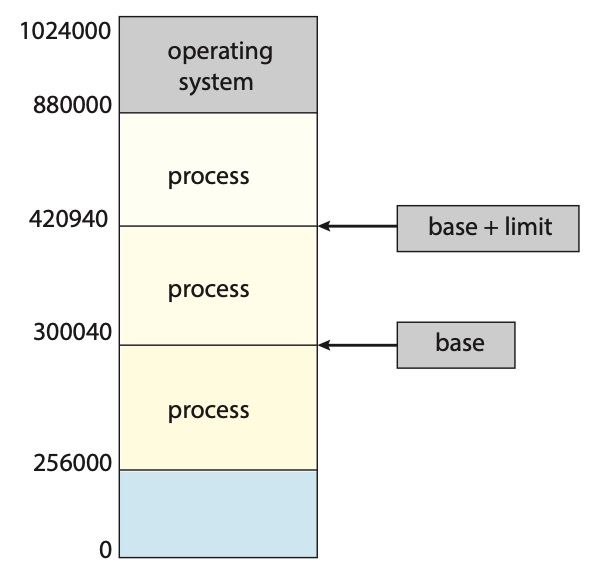
\includegraphics[width=0.3\linewidth]{assets/base-limit-memory.jpg}
\end{figure}

Nei sistemi moderni il processo può essere rilocato nella memoria a \textit{runtime}, questo grazie all'utilizzo della memoria virtuale. Questo ci permette di tradurre gli indirizzi fisici della memoria in indirizzi virtuali, non è quindi necessario allocare ad un programma un segmento contiguo di memoria, ma è possibile rendere contigui segmenti fisicamente lontani in memoria.

Questa traduzione avviene a livello hardware da parte della memory mapping and managment unit (MMU).

\begin{figure}[H]
    \centering
    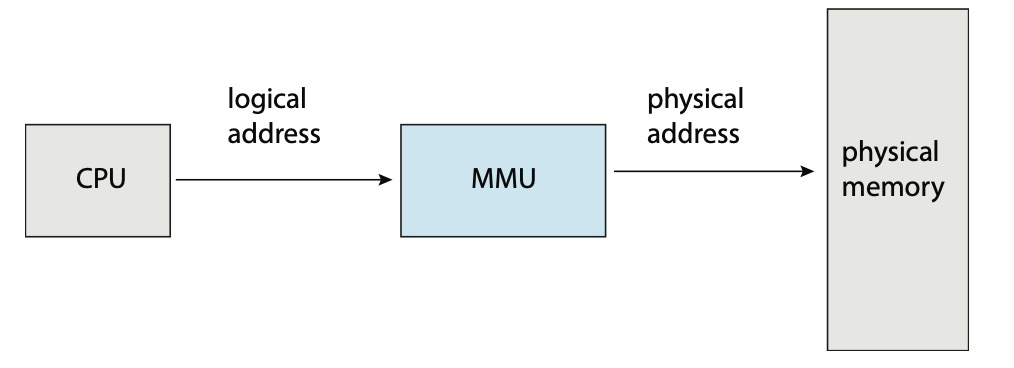
\includegraphics[width=0.45\linewidth]{assets/MMU.jpg}
\end{figure}

\subsubsection*{File di Paging}
Una funzionalità introdotta da Windows XP, che estende la memoria RAM del sistema con un file presente in memoria secondaria, delle stesse dimensioni.

\subsection{Frammentazione}
L'allocazione e la rimozione della memoria comporta la frammentazione della memoria.
\begin{sitemize}
    \item La \textbf{frammentazione interna}, quando la memoria allocata ad ogni programma è leggermente maggiore di quella richiesta.
    \item La \textbf{frammentazione esterna}, quando lo spazio per un nuovo processo è disponibile, ma non è contiguo, in questo caso può essere necessario rilocare dei processi per compattare lo spazio libero.
\end{sitemize}
